\documentclass{article}

\title{Temperature and the Santa Ana Sucker}
\author{Sophie Janssen and Nicole Larson}

\usepackage{Sweave}
\begin{document}
\Sconcordance{concordance:Report_Outline.tex:Report_Outline.Rnw:%
1 5 1 1 0 68 1}


\maketitle

\newpage
\tableofcontents
\newpage

\section{Introduction}

\subsection{Problem Statement}


\subsection{Background (Literature Review)}
From our background research, we found that many species of fish are affected by the temperature in their habitats. This is especiallly related to studies done in rivers with higher than normal temperatures, due to damming and/or climate change. Because the Santa Ana Sucker is not a very big river and is subjected to large influxes of treated wastewater from the Rialto Channel and the THE OTHER TREATMENT PLANT, we hypothesized that the temperature may be abnormal in the river and therefore could be restricting the Suckers to their preferred location, site 1 - The Plunge Pool. We found that there were indeed daily spikes and lows in temperature. Site 3 and Site 4 had especially dramatic spikes, with Site 4 fluctuating

\subsection{Objectives}
Our goal with this experiment was to find out whether or not temperature was affecting the population and/or livelihood of the Santa Ana Sucker in the Santa Ana River.

\subsection{Materials and Equipment}

4 HOBO Tidbit Water Temperature Data Logger,
1 Optic USB U-4 Base Station,
1 Coupler,
4 Green Garden stakes,
Red flags,
Yellow marking tape,
Free HOBOware software,
Transportation to and from the river,
Ice Bath

\subsection{Methods}

We will obtain four HOBO Tidbit water temperature Data Loggers to set up at the Rialto Channel at Agua Mansa (site 4), another at the point where the other discharge site meets the river (site 2), another just above that site (site 3), and a fourth in the pool where Suckers have previously been observed (site 1). Before going to the river, we programmed the loggers via our base station and the HOBOware software to collect water temperature data every 15 minutes. In order to start the data process, we put each logger into the coupler and pushed the level til the light was flashing. We then put them in the river by looping a garden stake through one, sticking it into the substrate, and securing it with rocks. We then put yellow marking tape on plants nearby and red flags along the bank to show where we left the main path. We repeated this for each site, making sure the loggers were secure and fairly hidden. After seven nights (for site 3) and eleven nights (for the other sites), we returned to the river and collected the loggers. In the lab, using the software, we loaded our data and transferred it to RStudio. Later, to calibrate the loggers, we put them in an ice bath for 6 minutes to ensure that the temperature settled around zero and each logger was measuring to the same temperature with the same accuracy.

\subsection{Site Descrition}

We evaluated the Santa Ana River between... near Colton, California (Figure \ref{SAR_Image}). 

\begin{figure}
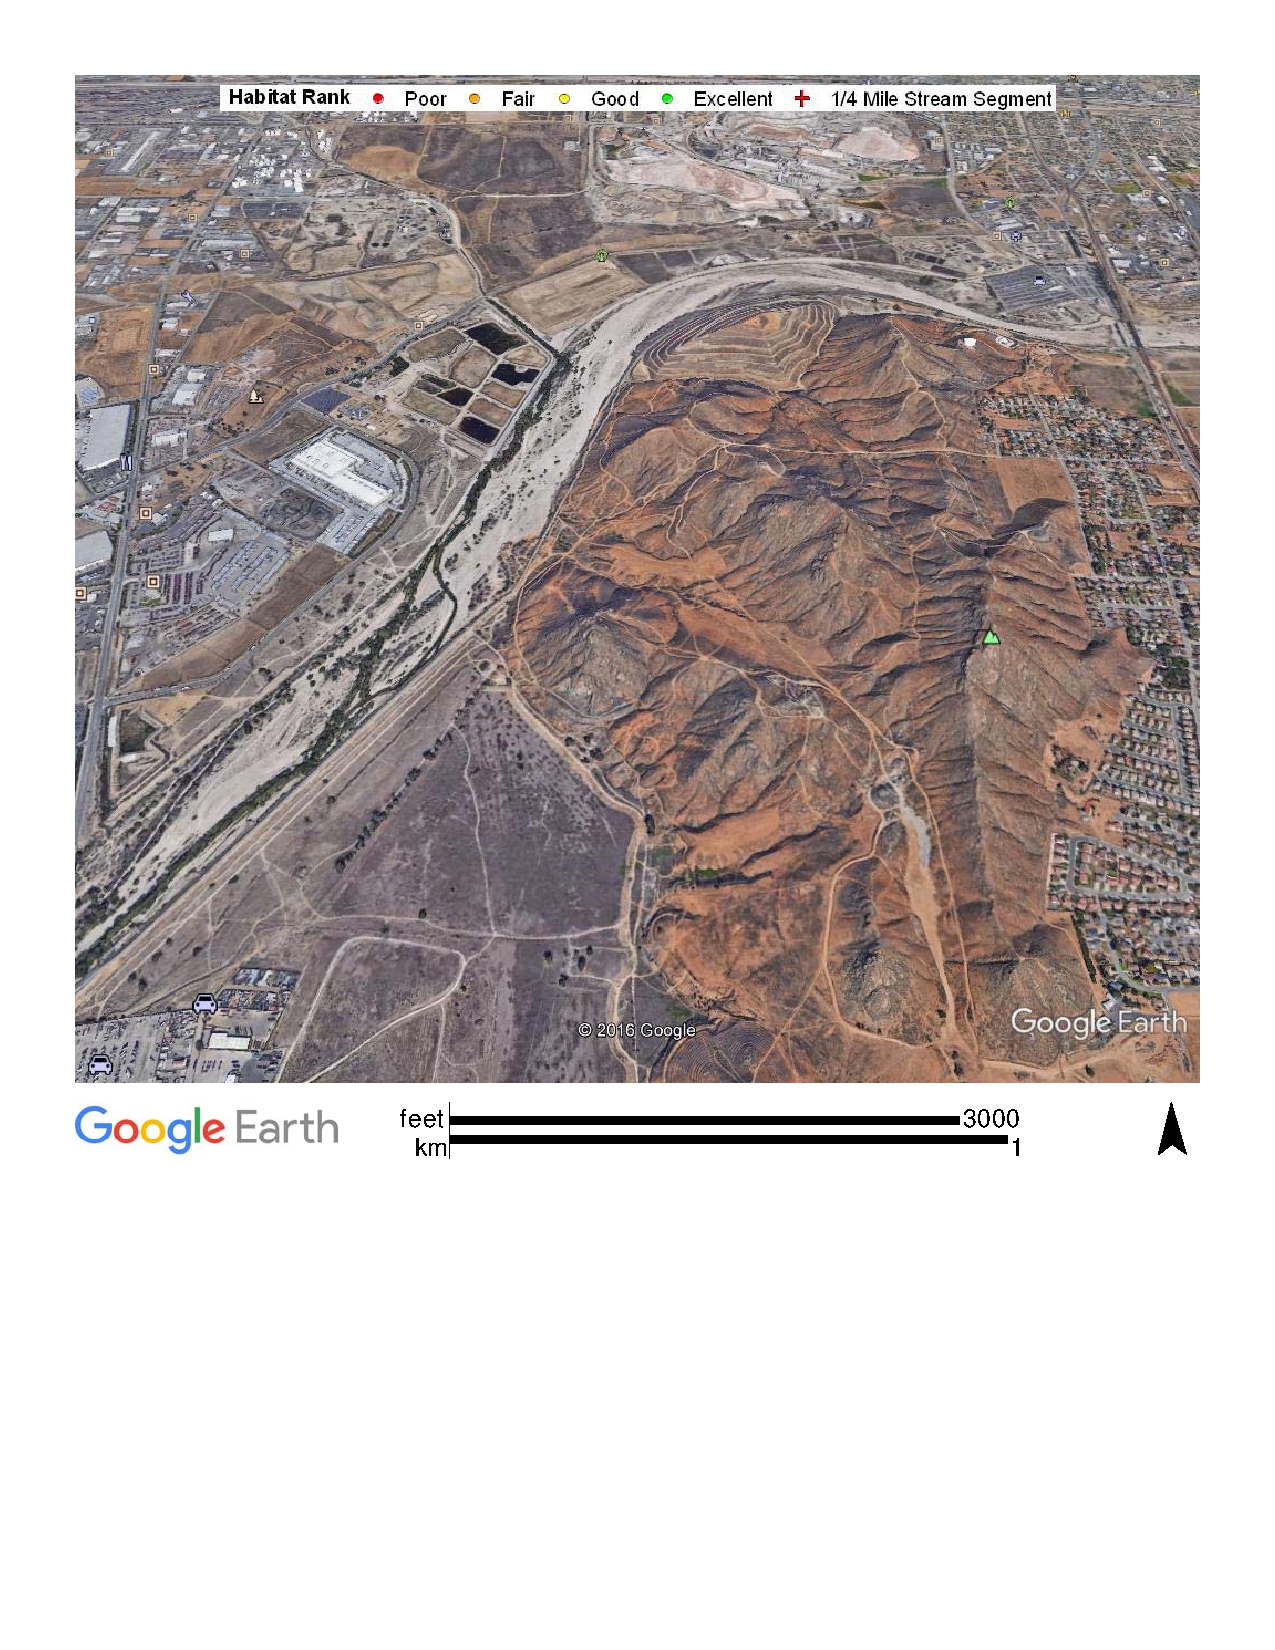
\includegraphics[width=1.00\textwidth]{Figures/SantaAna_SatelliteImage}
\caption{Google Earth --Example of a map. What's wrong with this image?}
\label{SAR_Image}
\end{figure}

\subsection{Field Methods}

\subsection{Laboratory Methods}

\subsection{Statistical Methods}

\section{Results}

The tempeature data suggests... (Figure \ref{Temp}).

\begin{figure}
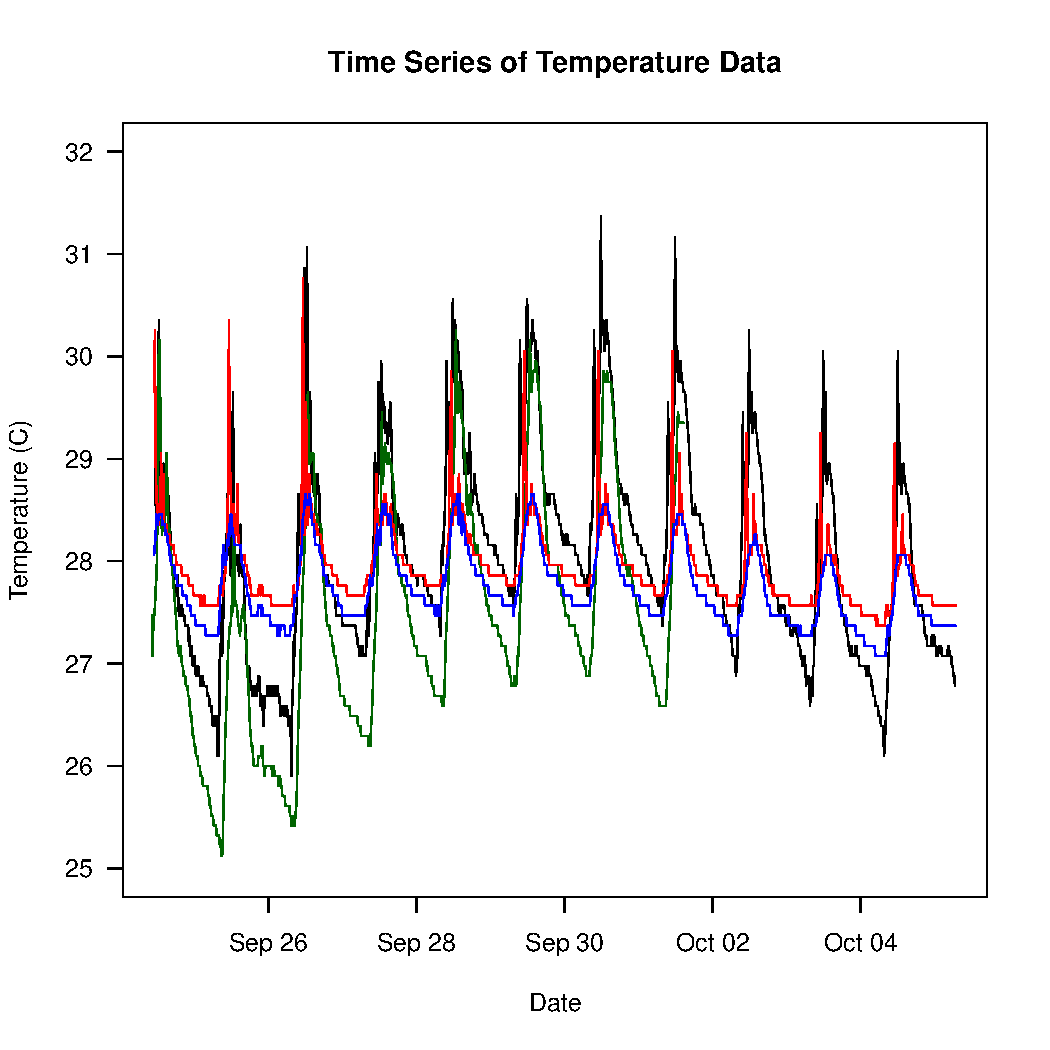
\includegraphics{Figures/Temp}
\caption{Temperature time...}
\label{Temp}
\end{figure}

\section{Discussion}


\section{Conclusion and Recommendations}


\end{document}
